% this file is called up by thesis.tex
% content in this file will be fed into the main document

\chapter{Fundamentals} % top level followed by section, subsection
This chapter explains basic theory of 3D reconstruction and Structure from Motion. All of this informations can be found in \cite{HartleyMultipleView}. Moreover it makes brief overview of sensor fusion made using accelerometer, gyroscope and magnetometer data. 

% ----------------------- contents from here ------------------------
\section{3-D reconstruction in general}
There are many possibilities of reconstruction from two-view reconstruction, multiple-view reconstruction to usage of stereo calibrated cameras like the ones used in Kinect[reference]. Reconstraction can be also performed with single hand-held camera either from video or images sequence. Only two images from different angles of one object are needed to perform 3D model generation. Reconstraction process consists of following steps:
\setlist[2]{noitemsep} % sets the itemsep and parsep for all level two lists to 0
\setenumerate{noitemsep} % sets no itemsep for enumerate lists only
\begin{enumerate}
\item \textbf{Image Acquistion}, where images are acquired 
\item \textbf{Feature extraction and correspondences matching}, where interesting features are extracted and compared between images
\item \textbf{Fundamental \& Essential Matrices} , where matrices satisfying basic epipolar geometry are calculated
\item \textbf{Camera parameters estimation} , where external and internal camera parameters are estimated
\item \textbf{Triangulation}, where camera projection matrices are composed and used in order to calculate 3D cloud points
\end{enumerate}
\subsection{Feature extraction and correspondence matching}
Usually each image used in reconstraction has to be analysed in order to find interesting features. Afterwards all of features in images are compared in order to acquire corresponding matches(\ref{fig:correspondingMatches}).
\begin{figure}[p]
    \centering
    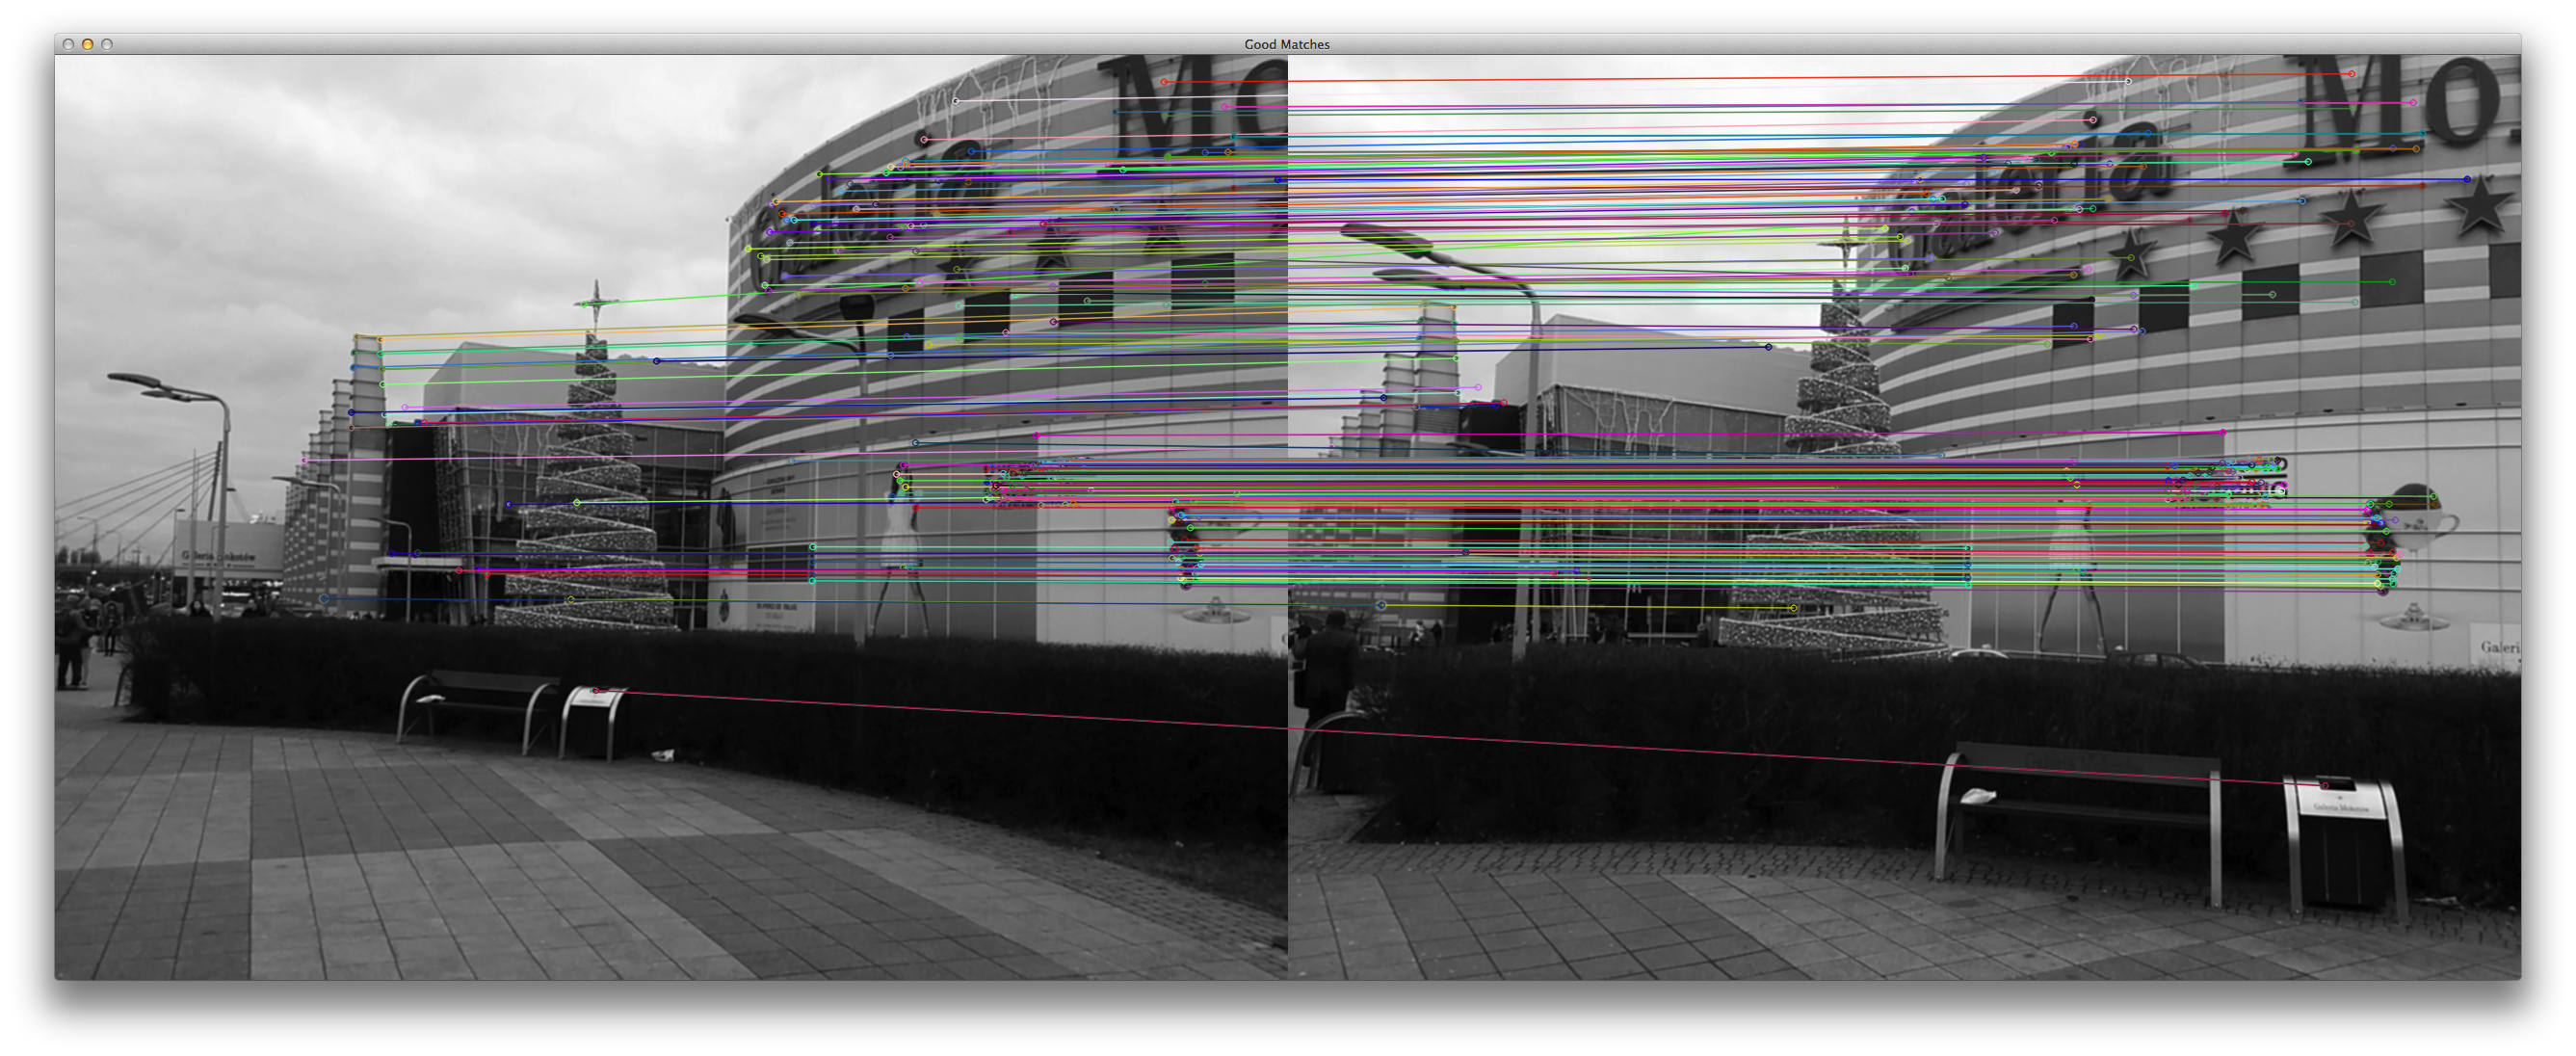
\includegraphics[width=0.8\textwidth]{correspondingMatching}
    \caption{}
    \label{fig:correspondingMatches}
\end{figure}
There are multiple features detector and extractors available to use \url{$http://en.wikipedia.org/wiki/Feature_detection_%28computer_vision%29$}. Some of them are better for edge detection, where others are better for corner or blob detection. One of the most popluar and robust feature detection method are Scale-invariant feature transform SIFT\url{http://en.wikipedia.org/wiki/Scale-invariant_feature_transform}. Using this descriptors local features in images are detected and described with metrics that are scale, rotation and translation invariant.
\subsection{Fundamental \& Essential Matrix estimations}
Once proper matches are decided, it can be proven that there exsists Fundamental matrix F for which following equation is satisfied:
\begin{equation} \label{eq:fundamntalEquation}
{x}^{'T} * F * x = 0
\end{equation} 
where $x$ and ${x}_{'}$ are uncalibrated points correspondances\cite{HartletMultipleView}TODO chapter. It is known that soultuions of this equation are highly sensetive to presence of outliers. Usually to make fundamental matrix estimations more accurate some outliers removing algorithms needs to be used. One of more robost approaches is usage of RANdom SAmple Consensus (\gls{ransac}) \url{http://en.wikipedia.org/wiki/RANSAC}. Sample fitting example can be seen in \ref{fig:RANSACFitting}
\begin{figure}[p]
    \centering
    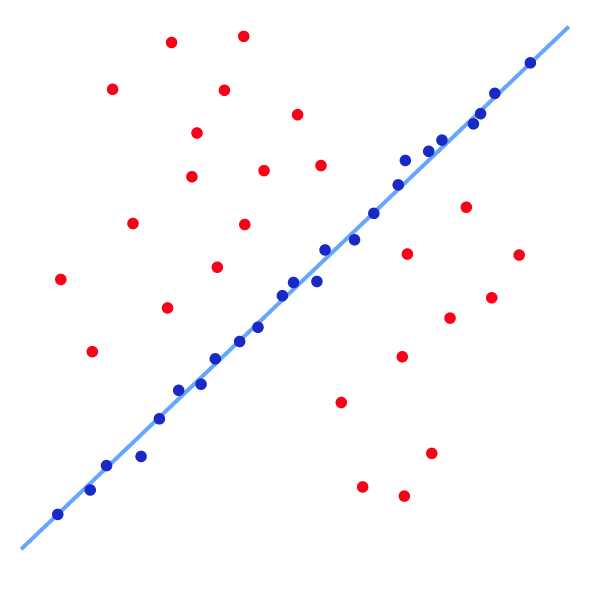
\includegraphics[width=0.8\textwidth]{RANSACFitting}
    \caption{Ransac fitting for 2D image}
    \label{fig:RANSACFitting}
\end{figure}
It basic idea relies on choosing randomly subset from whole correspondances, solving problem with reduced dataset and checking how many points from original set satisfies equation.
Using F epipolar lines for each point can be calculated(\ref{fig:EpipolarGeometry}). These lines crosses exactly same points in both images and can be used for dense feature matching as correspondances needs to be searched only in the neighbourhood of these lines.
\begin{figure}[p]
    \centering
    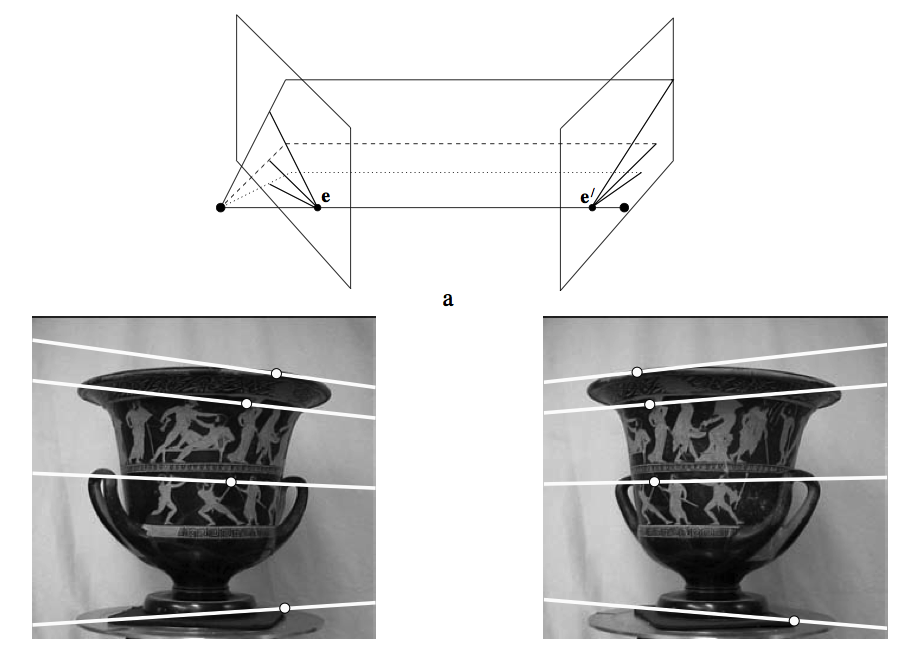
\includegraphics[width=0.8\textwidth]{EpipolarGeometry}
    \caption{Epipolar lines found in vase images}
    \label{fig:EpipolarGeometry}
\end{figure}
When enough inliers were found, points that didn't satisfy equation can be removed from further processing.
Once internal camera parameters K are known calculated image points can be calibrated and expressed in camera reference position system. Such calibrated points satisfy following essential matrix E equation:
\begin{equation} \label{eq:essentialEquation}
{x}_{c}^{'T} * E * x_{c} = 0
\end{equation} 
which is very similar to fundamental equation \ref{eq:fundamntalEquation}. This results in:
\begin{equation} \label{eq:essentialFundamentalRelation}
E = K^{T} * F * K
\end{equation} 
with $K$ being the internal camera parameters. Equation \ref{eq:essentialFundamentalRelation} is important in terms of decomposition of F to relative rotation and translation.
\subsection{Camera parameters estimations}
Internal camera parameters are expressed by following matrix:
\begin{equation}
\begin{bmatrix}
\alpha _{x} &  & x_{0} \\ 
 & \alpha _{y} & y_{0}\\ 
 &  & 1
\end{bmatrix}
\end{equation}
where αx = fmx and αy = fmy represent the focal length of the camera in terms of pixel dimensions in the x and y direction respectively. Similarly, x ̃0 = (x0,y0) is the principal point in terms of pixel dimensions. These parameters needs to be calculated only once for each camera model. Cameras can be calibrated with special reference boards of known dimensions and chracteristics.
In terms of propoer 3D reconstruction it is essential to properly estimate external camera parameters, such as rotation(orientation angles of the camera) and global postition of the camera. Usually in terms of 3D reconstraction these parametrs are not known. However in Chapter 9 of Multiple View Geometry in Computer Vision(\cite{HartleyMultipleView}) shows how essential matrix can be decomposed using Singular Value Decomposition \gls{svd} to relative camera positioning system of two projections:
\begin{equation}
 P1 = K * \begin{bmatrix}I\mid 0\end{bmatrix}
\end{equation}
second one is equall to 
\begin{equation}
 P2 = K * \begin{bmatrix}RDiff\mid tDiff\end{bmatrix}
\end{equation}
Unfortunately there are 4 possible solutions for such decomposition and it's not always possible to identify correct one.
\subsection{Points Triangulation}
Once internal and external(global or relative) parameters triangulation can be performed in order to acquire up to affine reconstruction model (\ref{eq:3Dreconstruction}).
\begin{figure}[p]
    \centering
    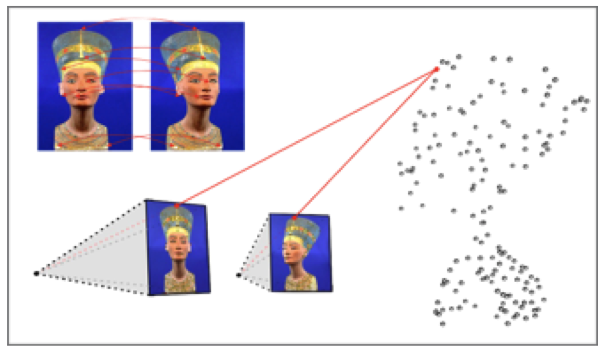
\includegraphics[width=0.8\textwidth]{3Dreconstruction}
    \caption{}
    \label{fig:3Dreconstruction}
\end{figure}
Only scale factor cannot be determined in such relative case situation. In [TODO hartley chapter 10] this process is described in details.
\section{Structure from Motion}
Term of Structure from Motion(SfM) refers to structure reconstraction from consecutive sequences of moving camera. It is really popular research topic and two main different approaches called Pose Estimation and Homography Estimation can be used to make it happen.
\subsection{3D Pose Estimation}
Assuming that some 3D cloud point is already known, correspondences between 2D features in new image and 3D point clouds positions can be established. Such 3D-2D correspondences can be used to estimate next camera relative to model position. This allows of reconstraction of new 3D points and merging them smoothly into existing model. Unfortunately this process is also highly sensitive to presence of outliers, so adequate measeures has to be made in order to reduce their influence. One of the main advanteges this method is speed, but on the other hand it's effectiveness strongly relies on exising 3D cloud quality. 
\subsection{Homography estimation}
New image can be reconstructed with previous once in a standard way to recive up to scale 3D model. Later freshly acquired model can be merged to existing one using Homography estimation between coresponding 3D points. Such strategy is slowet than previous, but it is not influenced by quality of existing 3D model. It's also higly sensitive to outliers, but once made accurately produces much more new 3D points.
\subsection{Structure Adjustment}
After some time of SfM reconstruction some techniques, which compensate increasing error of wrong estimates propagating through images special algorithms can be used to refine reconstructed models. One of such techniques is Bundle Adjustment\gls{ba} \url{http://en.wikipedia.org/wiki/Bundle_adjustment}. Through finding point correspondances between multiple sets of images algorithm iterativly modifies either both of one camera external paramaters as well as 3D points positions. It's main disadvantages is execution times. It takes a lot of time to use it in real-time applications. In figure \ref{fig:BundleAdjustment} basic idea of BA is expresed.
\begin{figure}[p]
    \centering
    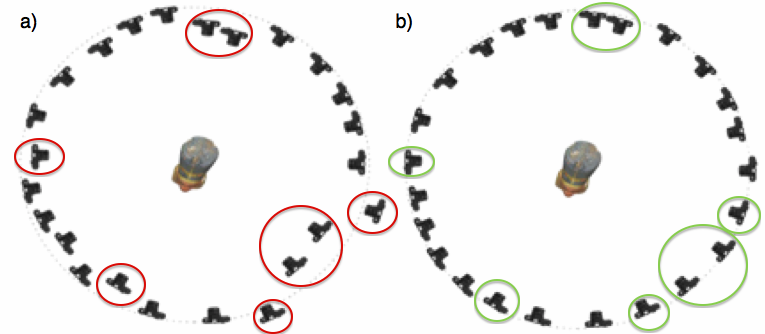
\includegraphics[width=0.8\textwidth]{BundleAdjustment}
    \caption{}
    \label{fig:BundleAdjustment}
\end{figure}
\section{Mobile Sensors overview}
There are many sensors available in nowadays smartphones such as accelerometer, gyroscope, magnetomere, barometer, GPS etc. All of them have their advanteges and disadvanteges, but their errors, different in nature, can be compansated with each other to for exmaple accuretly compute camera rotation angles.
\subsection{Accelerometer}
An accelerometer is a device that measures acceleration along 3 axes of the device[reference]. Generally, accelerometers alows to measure total acceleration by sensing how much mass presses on its micro strings when a force is applied. An accelerometer, which lay on a flat surface perpendicular to the Earth's surface will indicate approximately 1G upwards. This gravitation vector can be used to caculate relative camera rotation, but it's hard to tell where in which direction gravity vector points, when device is moving in not linear manner. To obtain the gravity vector and track it during unexpected movement gyroscope sensor can be used.
\subsection{Gyroscope}
A gyroscope is a device for measuring or maintaining orientation, based on the principles of conservation of angular momentum [reference]. A standard gyroscope consists of a spinning wheel mounted on two gimbal rings, which allow it to rotate in all three axes. The spinning wheel will resist changes in orientation, due to an effect of the conservation of angular momentum. A conventional gyroscope measures orientation, in contrast to MEMS (Micro Electro-Mechanical System) types, which measure
angular rate, and are therefore called rate-gyros [reference]. MEMS gyroscopes contain vibrating elements to measure the Coriolis effect. In the end the angular velocity can be calculated in each axis. It is important to note that whereas the accelerometer and the magnetometer measure acceleration and angle relative to the Earth, gyroscope measures angular velocity
relative to the body.
\subsection{Magnetometer}
A magnetometer is an instrument used to measure the strength and/or direction of the magnetic field in the surrounding area of the instrument. It's main idea works the same as conventional compass. With some magentometers magnetic field can be me in 3 particular directions, relative to the spatial orientation of the device [reference]. Using magnetometers allows for relative position estimation in geomagnetic north position system. 
\subsection{Sensor Fusion}
Sensor fusion is the process of  combining sensory data derived from sensory data from disparate
sources such that the resulting information is in some sense better than would be possible
when these sources were used individually. The term better in this case can mean more
accurate, more complete, or more dependable, or refer to the result of an emerging view, such
as stereoscopic vision (calculation of depth information by combining two-dimensional
images from two cameras at slightly different viewpoints) [reference]. One of the possible strategies is Kalman-filterring(\ref{fig:Kalmann})
\begin{figure}[p]
    \centering
    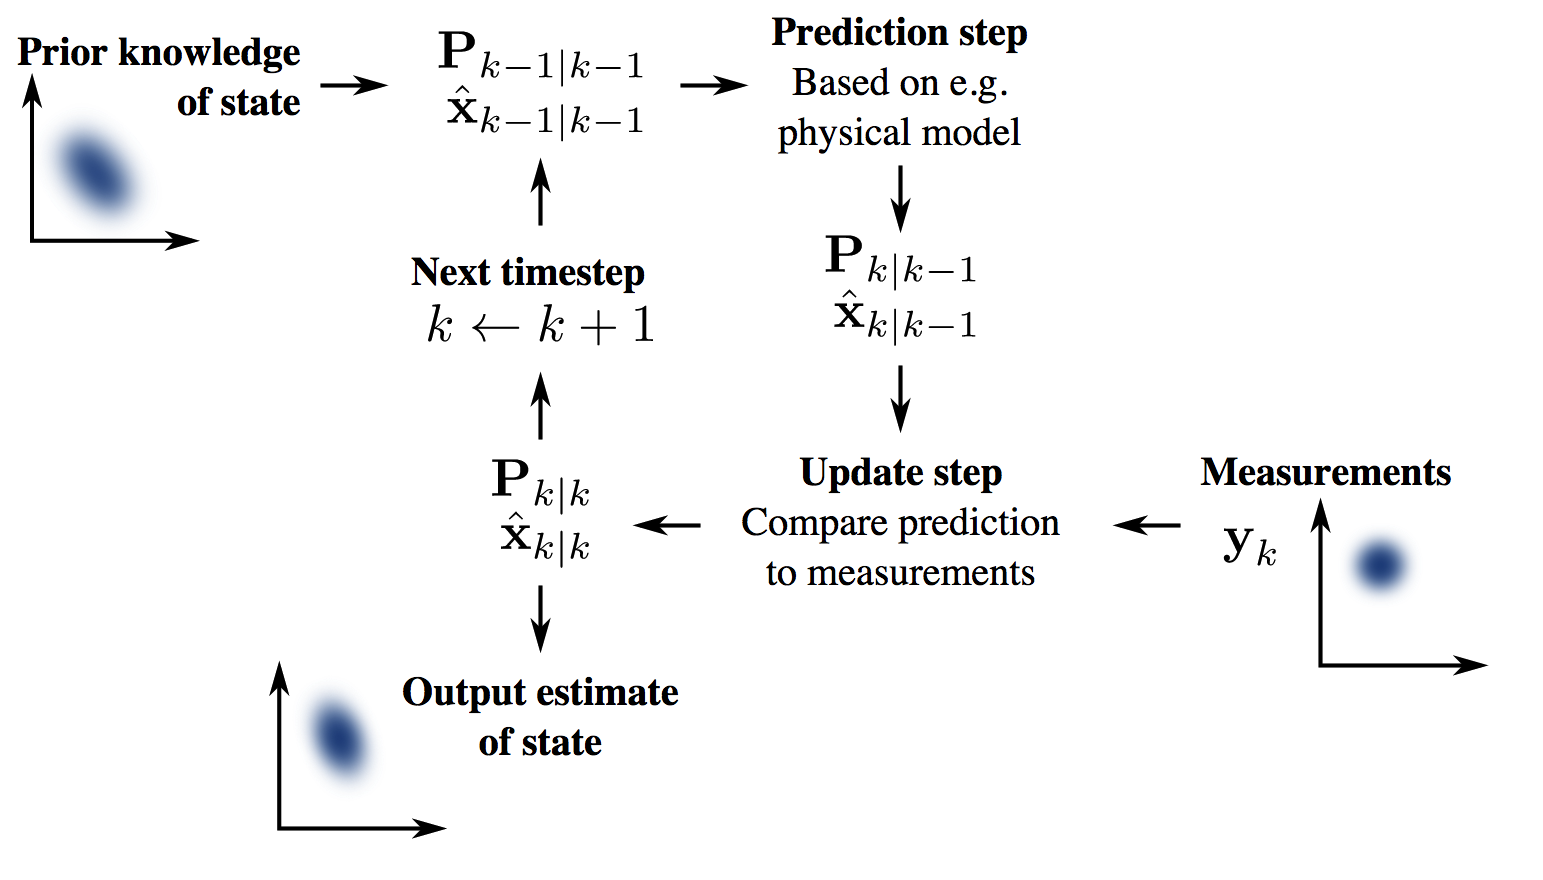
\includegraphics[width=0.8\textwidth]{Kalmann}
    \caption{}
    \label{fig:Kalmann}
\end{figure}
Available in Android API SesnorFusion sensor uses this approach, where the base of orientation measurements is calculation of gravity, when device was not moving and using gyroscope data (very accurate for a short period of time), when device starts to unexpectedly moving. Magnetometer data are fusined to allow for global earth coordinate system.


% ---------------------------------------------------------------------------
% ----------------------- end of thesis sub-document ------------------------
% ---------------------------------------------------------------------------